\chapter{Language Interpreter Design}


\section{Imperative and Declarative language}




\section{Type System}
\subsection{Dynamic Typing and Static Typing}
A programming language is said to use static typing when type checking is performed during compile-time as opposed to run-time. 
For example , you have to specify the type explicitly and the compile will the the type correctness of a variable.A variable of a specified type can not assign to another value of other type.

\begin{tabular}{p{5cm}|p{5cm}}
\hline
Static Typing & Dynamic Typing \\
\hline
int a =1;\par \textbf{/*a is of type int */} \par int a="a string"; \par \textbf{ /* its not valid to assign a string to a variable that has type int */} & a=1; \par \textbf{/* does not need to specified a type for this variable */} \par a ="a string"; \par
\textbf{/* it valid to change the type of the variable */} \\ 
\hline
\end{tabular} \\\\
In my project, I used the dynamic typing scheme,which is ,does not need to specify any type of variable and able to assign any type of primitives to a variable.

\subsection{Strong Typing and Weak Typing}
a language is said to be strong typing is that it place restriction in operation where data type can not be intermix.


\begin{tabular}{p{6cm}|p{6cm}}
\hline Strong Typing & Weak Typing  \\ 
\hline a=123; \par 
\textbf{/* a is a number */} \par 
b="123" \par  
\textbf{/* b is a string */} \par 
c=a+b \textbf{/* return type error */}  &  
a = 123; \par 
b = "123"; \par
c = a+b; \par 
\textbf{/* either a will be convert to a string or b will be convert to a number */}

\\ 
\hline 
\end{tabular} 

In my project,I have implemented a weak typing system .I have design an statement call generic expression , which allow different kinds of value to intermix with each other. An expression like "12343" + 1232 -324 can be parse as follow syntax tree.




\section{Problem and resolution in writing BNF/EBNF rules}
\subsection{Shift//Reduce Problem}

\subsection{Reduce//Reduce Problem}

\section{Syntax Design}

\subsection{The Main Structure}
A module is the minimum executable unit in \textbf{yun}.It is composed by one main function and serveral functions.The main function is a entry point,it may invoke other functions.

\begin{figure}[h!]
  \centering
	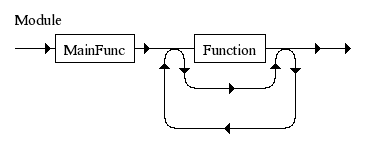
\includegraphics[width=0.90\textwidth]{pic/c4/module.png}
	\caption{Module Syntax Diagram}
\end{figure}

\begin{figure}[h!]
  \centering
	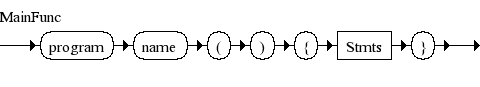
\includegraphics[width=0.90\textwidth]{pic/c4/main_function.png}
	\caption{Main Function Syntax Diagram}
\end{figure}

\begin{figure}[h!]
  \centering
	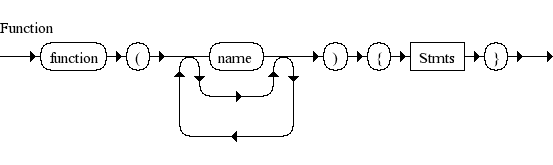
\includegraphics[width=1.00\textwidth]{pic/c4/function.png}
	\caption{Function Syntax Diagram}
\end{figure}


Possible program code may looks like follow,

\begin{lstlisting}[language=java]
program main ()
{
 	result = sum(1,2,3);
 	// more code
 	
}


function sum (var1,var2,var3)
{
	// body of the functions
}

// may be more functions
\end{lstlisting}


\subsection{Statements}
Statements  comprise the body of a function.A statement may be a assignment,break and continue sentence,return sentence.WhileBlocks ,IfBlocks,ForBlocks are all statements.What's more , WhilcBlock,IfBlock,ForBlock are recursively defined by statements as well.This allow nested for loop ,nested while loop and etc.

\begin{figure}[h!]
  \centering
	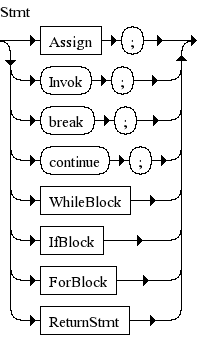
\includegraphics[width=0.45\textwidth]{pic/c4/stmt.png}
	\caption{Statement Syntax Diagram}
\end{figure}

The following code can be consider as a statement of the language
\begin{lstlisting}[language=java]
while ()
{
} /* the while statement */

if ()
{
}
else
{
} // the if else statement

for ( )
{
	for ()
	{
	}
} // nested for loop 


a = 1 ; // assignment statement, assign a value or and an expression to a variable

fib(5);  // function invocation statement


\end{lstlisting}

\subsubsection{Assignment}
There are three type of assignment in the language .They are ,
\begin{itemize}
\item Function invocation assignment.Assign the return result to a variable.
\item Generic expression assignment.Assign the result of an expression to a variable.
\item List assignment.Assign a list to a variable.
\end{itemize}
As \textbf{yun} is an imperative language,the right side of the assignment operator will be evaluation immediately. In other word,the language is strict.



\begin{figure}[h!]
  \centering
	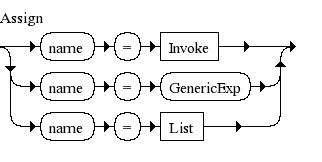
\includegraphics[width=0.65\textwidth]{pic/c4/assign.png}
	\caption{Assign Statement Syntax Diagram}
\end{figure}

\subsection{Generic Expression}



